\chapter{Team 3 Agent Design}

\title{Team 3: Pittstop Agent Strategy}

\maketitle

\section{Introduction}

Team 3 was interested in the parallels between this project and human societies. We wanted to build an agent that was flexible enough to mimic the diverse personality traits of ordinary citizens, as well leaders in governments around the world.

Section~\ref{sec:overall_strat} discusses the foundation of parameters and methods the team wrote in its approach towards building the agent. Section~\ref{section_func_team3} details how the team used this foundation to implement the required functionality of the agent (i.e. roles, voting, prediction, gifting, foraging) in a way that is compatible with our goal of flexibility, without compromising efficiency or intelligence. Section~\ref{sec:team3_simulation} then elaborates on game simulations, in which the team decided to anthropomorphize the agent by modelling it after three famous historical and political personalities. Simulations consisting of different permutations of these personalities reveal interesting conclusions about the performance of the archipelago. Finally, Section~\ref{sec:management} concludes our report with information about project management.

\section{Overall Agent Strategy}
\label{sec:overall_strat}

\subsection{Overview}
\label{sec:overview}


The agent was created by first a set of high-level parameters, most of which were used as scaling factors throughout the code base of the agent, and some as Boolean values that turn on or off specific behaviours. These parameters hence govern the agents interactions with the rest of the game. The effect of each parameter on the behaviour of the agent is summarized in Table~\ref{tab:team3:parameter_effects}. \\


\begin{center}
    
\begin{table}[H]
\centering
\begin{tabular}{l|l}
\textbf{Parameters} & \textbf{Description}  \\ 
\hline
\texttt{equity}                       & controls the allocation distribution of resources amongst islands              \\ \hdashline
\texttt{resourceSkew}                 & factor to adjust resource allocation based on trust             \\ \hdashline
\texttt{complianceLevel}              & quantifies how often the agent cheata during the game             \\ \hdashline
\texttt{saveCriticalIsland}           & if True, our agent will try to save any critical island             \\ \hdashline
\texttt{selfishness}                  & quantifies how selfish our agent is (e.g. in the context of gifts)             \\ \hdashline
\texttt{riskFactor}                   & quantifies how much risk our agent is willing to take        \\ \hdashline
\texttt{friendliness}                 & quantifies how friendly we will be during agent interactions            \\ \hdashline
\texttt{sensitivity}                  & quantifies how sensitive the agent will be to external changes            \\ \hdashline
\texttt{giftInflationPercentage}      & factor to adjust when gift requests are made to other islands             \\ \hdashline
\texttt{advType}                      & enables the agent to exploit institutional powers when elected in a role    \\ \hdashline
\texttt{controlLoop}                  & boolean to enable the feedback loop for the agent       
\end{tabular}
\caption{List of global parameters that dictate our agent strategy.}
\label{tab:team3:parameter_effects}
\end{table}
\end{center}

\subsection{Core functions}

Based on these parameters, we also wrote a set of core functions which would be useful to all variations of the agent. These functions implement Opinion Formation and Compliance Calculation.


\subsubsection*{Opinion Formation} \label{section_opinion_formation}
In a game where there can be up to n-agents, \textit{opinion formation} allows our agent to quantitatively assess the behaviour of the others based on previous interactions. %The agent uses this information in the form of \textit{trust decision-making} to reduce uncertainties and ultimately maximise its returns during any activity. 
In our implementation, we use a \texttt{trustScore} map to keep track of the agent's trust in (n-1)-agents. This map is used in combination with other pre-configured parameters to make strategic decisions during a turn. 
Trust takes a score between 0 (lowest) and 100 (highest). At the beginning of the game, all trust scores are initialised at 50, representing a neutral opinion. In our implementation, the trust scores can change during the following game activities:

\begin{itemize}
    \item Gifting: When our agent receives gift offers (after requesting gifts) and actual gift amount(s) received.
    \item Role Evaluations: When our agent evaluates the performance of the President, the Speaker and the Judge based on their respective roles and responsibilities.
    \item Sanctions: When we receive the broadcast of sanction from the Judge outlining the sanctions placed for that turn.
\end{itemize}

%This mean that the more turns there are in a game, the more variation one will observe in the trust scores. They provide an effective source of perceived opinion for the agent to intelligently devise and choose a strategy in a given situation with limited external information. 

At every turn of the game, the agent will participate in multiple activities and hence, it would be counter-intuitive if the agent directly updated the \texttt{trustScore} map otherwise only the last score change would be retained. We thus implemented a local cache, \texttt{trustMapAgg}, to keep track of all trust score updates made during agent activities for that turn. 

In the following turn, the \texttt{trustScore} map is updated by averaging all cached trust score changes for each agent in play. This allows the agent to progressively accumulate knowledge while still forming independent opinions from the results of the activities in each turn. Trust scores are also bounded between 0 and 100 for consistency. The process (for a single turn) is summarized in Figure~\ref{fig:trust_scores}.\\

\begin{figure}[H] 
\centering
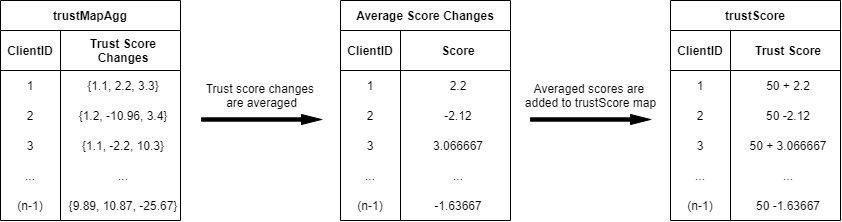
\includegraphics[width=0.75\textwidth]{11_team3_agentdesign/figures/TrustScores.jpg}
\caption{Diagram showing the series of changes to trust scores during a single turn.}
\label{fig:trust_scores}
\end{figure}

%The \texttt{trustScore}  For example, when our island is elected as a Judge, the agent will rely upon these trust scores to determine which islands to pardon. This allows the agent to facilitate trust and forgiveness within the same framework.

\subsubsection*{Compliance Calculation}
Compliance Calculation determines at what point of the game it is most strategic to cheat. At every turn we calculate the \texttt{compliance} for the next turn\footnote{Note that \texttt{compliance} is how much our agent should comply at a given turn, while \texttt{complianceLevel} is how much our agent should comply during the entire game.}. The compliance calculation is based on the following principles:
\begin{enumerate}
    \item Every time we are caught, \texttt{compliance} is reset to 1.
    \item The more our agent is caught, the less it should cheat.
    \item If our agent has not been caught cheating for an infinite amount of turns, $\texttt{compliance}=\texttt{complianceLevel}$.
    \item The more our agent is caught, the longer it should take \texttt{compliance} to converge to \texttt{complianceLevel}.
\end{enumerate}

Those principles were converted into Equation~\ref{team3:eq:compliance}, shown here below:

\begin{equation}
    c(t,n)=\texttt{complianceLevel}+(1-\texttt{complianceLevel})\times e^{\frac{-t}{n+1}} \label{team3:eq:compliance}
\end{equation}

where:
\begin{conditions}
 c     &  \texttt{compliance} at a given turn \\
 t     &  time since the agent was last caught by a Judge (in number of turns) \\
 n    &  number of times the agent has been caught since the game started \\   
 \texttt{complianceLevel} &  target compliance - global parameters (see Table~\ref{tab:team3:parameter_effects})
\end{conditions}

Figure~\ref{fig:compliance_decay} illustrates how compliance decays based on the number of times caught. 

\begin{figure}[H] 
\centering
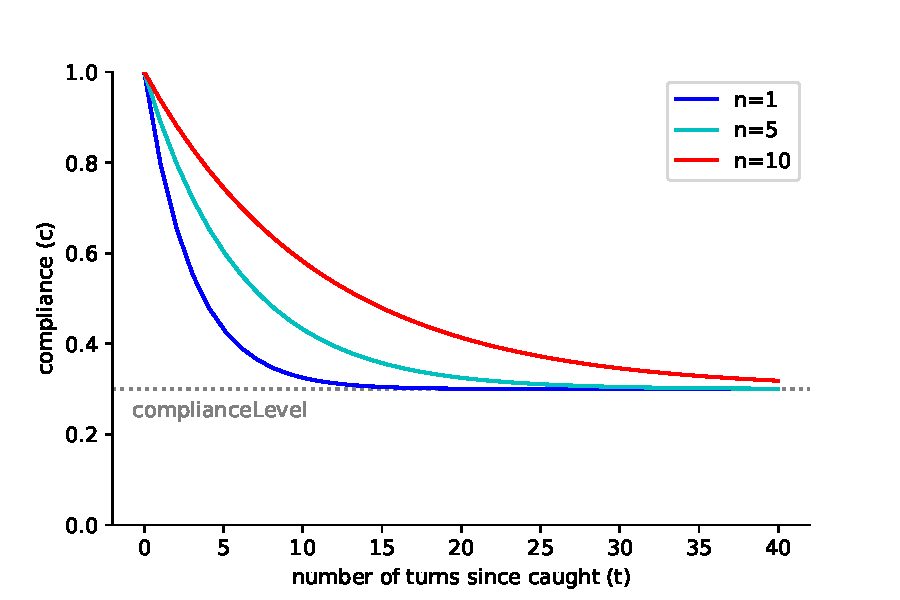
\includegraphics[width=0.4\textwidth]{11_team3_agentdesign/figures/compliance_graph.pdf}
\caption{Compliance decay over several turns with $\texttt{complianceLevel}=0.3$.}
\label{fig:compliance_decay}
\end{figure} 

The agent, in various functions described in the following section, then decides whether or not to cheat by generating a random real number in $[0,1]$ and checking if it is lower than \texttt{compliance}.

% \begin{center}
%     \text{Let $X$ be a random number between 0 and 1,}
% \end{center}
% \begin{equation}
%   i.e.  X \sim U( [0,1]).
% \end{equation}

% \begin{equation}
%     if \; \texttt{compliance} < X \rightarrow \; cheat
%     \label{eq:should_I_cheat}
% \end{equation}

\subsubsection{Common State Variables}
In addition to the global parameters, a number of variables were also created to track the current state of the agent. These are accessed and updated by most functions throughout the agent's code base. 
\begin{itemize}
\item Gifting history
\item Trust scores for each island 
\item Performance score of each island for positions of power (i.e. the Speaker, Judge, President)
\item Number of times sanctioned
\item Cached information from IIGO (e.g. sanctions, monitoring outcomes and taxation/allocation)
\end{itemize}

\section{Implementation of agent-specific functions}
\label{section_func_team3}

This section covers how we implemented functions for each of the expected behaviours of the agent, as well as details of how they are affected by parameter changes.

\subsection{Voting}

\subsubsection{Voting for Rules}
Our rules are stored in the form of matrices, which opens up to our agent the geometric analysis of linear algebra. We observe that each rule matrix requires a number of inputs. These inputs may be considered to form $n-dimensional$ space. \\
As explained in Section~\ref{dynamics} below, our dynamics package is able to analyse these n-dimensional spaces and calculate whether a particular rule pushes us further from compliance or moves us towards a compliant position in this $n-dimensional$ space. Depending on whether the proposed rule brings us closer to compliance or not, we chose to vote for or against it.

\subsubsection{Voting for Elections}
At the end of each session of the IIGO, all islands need to submit votes for their preferences for the next Speaker, Judge and President. Since the vote is implemented using a Borda Count, teams are required to submit an ordered list of islands, ranked according to preference. 

We implemented voting by evaluating the performance of each island that held the positions of Speaker, Judge and President at the end of each IIGO session. Evaluations are performed using heuristics. Islands are ranked for each role based on the report from the accountability cycle and our interaction with the role during the turn. For example, if the Speaker chose the rule we suggested, they would have a better evaluation. However, if we get a smaller than requested allocation from the President, we would rank the island occupying the role lower.

\subsection{Environment}

\subsubsection{Foraging}
Foraging for our agent was implemented to maximise the return while maintaining a risk proportional to the \texttt{riskFactor} parameter. To achieve this, we use foraging results from previous turn from our island and the ones shared by other islands in  IIFO.
Our foraging strategy decision making ensures we are not in a critical state if foraging does not turn profitable.

At every turn, we follow the following strategy:

\begin{enumerate}
    \item Determine maximum foraging investment amount amount using the \texttt{riskFactor} parameter, our current resources and our estimation of the critical threshold.
    \item Set the maximum foraging investment amount based on our current resources and the minimum leftover resources amount.
    \item Compute the expected return of investment of both foraging techniques, hunting and fishing, using the stored history of past foraging returns. 
    \item If one foraging technique has a positive expected return, we compute a decay factor to adjust our investment based on what islands have chosen to forage in the last turn and how many dears/fishes were caught. This ensures that we do not hunt when the population is too low or that a lot of other islands are foraging with us.
    \item If no foraging technique is expected to be profitable, we only invest a small amount to get additional information in the next rounds and we don't take unnecessary risks.  
    \item The final amount we decide to forage is scaled by the risk factor parameter.
\end{enumerate}

This foraging decision making algorithm proved to be efficient and produces stable positive returns at different risk levels for our agent.

\subsubsection{Disaster Prediction}

Our agent predicts disaster using a combination of our own estimation of the disasters distribution and predictions from other teams.

Our estimation is obtained by computing the mean and variance of the coordinates, the magnitudes and the number of turns between past disasters. The variance is used to specify the confidence we have in our own prediction.

Other island's predictions are weighted based on their forecasting ability obtained by analysing their history of predictions of past disasters, the confidence they have in their own predictions as well as how much we trust them.

At each turn, we share our predictions with alive islands and store the ones from other teams. When a disaster occurs, we log this information to determine forecasting abilities of other islands.

\subsection{Trade}

The gifting session described provides four major phases for our agent to take part in. Trade is a two-way interaction and as per game sequence, it is the first opportunity (in every turn) to formulate an opinion.

\subsubsection{Gift Requests}
Our gift requests depend on 2 main parameters in our agent strategy, \texttt{giftInflationPercentage} and \texttt{riskFactor}, along with the \texttt{trustScore} map that we have built based on opinion formation of the other island. Essentially, we cover the risk that we do not get resources from the islands that we do not trust as much with what we get from islands that we do trust. Additionally, we do not request any gifts from critical islands in order to help them survive. \\

At every turn, we follow the following strategy:

\begin{enumerate}
    \item The resources our islands plans to ask for in gifts is calculated by finding the different between the \texttt{initialResourcesAtStartOfGame} and our \texttt{localPool}.
    \item If we actually need resources, we inflate the total requests that we make to account for differences in gifts we might actually receive. Otherwise, if do not actually need resources, we just request a percentage of \texttt{initialResourcesAtStartOfGame} for later opinion formation.
    \item We find the number of alive islands in the game and calculate the average amount of resources we will be requesting from each of them based on our total number of resources we wanted in the previous step.
    \item If an island is critical or dead, we do not request any gifts from them. For all other islands, we use the average request amount and adjust it according to \texttt{trustScore} of the island raised to the power of our island's \texttt{riskFactor}.
\end{enumerate}

\subsubsection{Gift Offers}
We make gift offers based on the other islands' gift requests, their respective \texttt{trustScores}, and some of our agent's parameters such as \texttt{friendliness} and \texttt{selfishness}. However, if our island is critical, we do not many make any offers so that we can stay alive, but if our island's local pool resources are less than 10\% of \texttt{initialResourcesAtStartOfGame}, we still make a $0.01$ amount of gift offer to all alive islands. Our main strategy is to give as many gifts to the islands to maintain a good relationship with them.\\

In all other circumstances, we process the \texttt{receivedRequests} in the following manner:

\begin{enumerate}
    \item We use a sigmoid function to distribute and normalise the requests we receive from other islands based on their trustScore. More specifically, we use the following equation:
    \begin{equation}
    sigmoid = \frac{1}{1+e^{-0.1*(trustScore[island]-50)}}
    \end{equation}
    and normalise it so that the number is between 0 to 100, and then multiply it with the original request to scale the amount we are thinking of offering them. In this way, we offer less to islands that we trust less and more to islands we trust more.
    \item Calculate our gift budget based on \(\texttt{localPool}*(1-\texttt{selfishness}/2)\).
    \item Rank the islands based on their trust score in descending order.
    \item Allocate the gift offers starting from the most trustworthy islands onwards, until we run out of our gift budget.
\end{enumerate}

Lastly, when we actually send the gifts to other islands at the end of each turn, we inflate our gift offers to improve other islands' opinion of us.

\subsubsection{Gift Responses}
We accept all amounts of gifts that the other islands offer us. The only exception to this is when the offering island is critical, then we do not take any of their offered amount in an attempt to conserve their resources as much as possible and increase their chances of survival as part of the common risk dilemma.

\subsubsection{Updating Gift History}
We use this section of gifting to do some opinion formation of other teams and more specifically update our \texttt{trustScore} map. If our offered gifts are declined or ignored with the reasons \texttt{DeclinedDontLikeYou} or \texttt{Ignored}, then we decrease that island's trust score by 5 and 2.5 respectively. When we actually receive our gifts, we compare the received amount to what we originally requested from an island, and use the difference to increase their trust score if they gave us more than we asked for or decrease it (with the exception of if the island is critical) if they gave us less.

\subsection{Taxation and Allocation}
%TODO: might need to move this for better organisation
\subsubsection*{Paying Our Taxation Amount}
Our taxation paying system has the similar aim as our President's tax allocation system. It aims to ensure that common pool has enough resources to survive the upcoming the disasters as well as run the next IIGO session. This is done based on the main assumption that each islands would probably pay proportionately to the trust that our agent has on them as well as others having the same aim as the agent's. This algorithm depends on \texttt{selfishness} and \texttt{riskFactor}.\\

At every turn, we follow the following strategy:

\begin{enumerate}
    \item Minimum resources that common pool should be is calculated based on the predicted disasters incoming as well as the cost of running IIGO.
    \item Distribute the share of the payment based on the trust on them, with the agent's own trust being represented by 1-\texttt{selfishness}.
    \item Calculate the minimum amount of resources the agent should have, this depends on the \texttt{riskfactor}. 
    \item Ensure that the taxation amount will not put the agent below the minimum resources. 
    \item Depending on our compliance level, if our calculated amount is lower than our given taxation, we will increase it accordingly.
\end{enumerate}


\subsection{Positions of Power}

\subsubsection{Judge}

% The judicial branch references the functionalities an island can implement if they are elected as the Judge. 
The overall strategy for our island as the Judge was to enforce stricter laws to encourage more obedience (in the future) from the other agents while respecting the power, permission and obligation paradigms. 

\subsubsection*{Inspect History}
To respect the role of the Judge, our client performs the inspection as per base Judge implementation (i.e. evaluates if rules were followed by all islands) with the exception that our and other highly trusted islands (whose trust score is above 80) are exempted from all evaluations. A false evaluation map indicating full compliance with rules is produced for these cases and a correct evaluation is produced for all the other islands. 

% \subsubsection*{Rule Violation Severity}
% Our agent does not override these severities because we did not have sufficient opinion formation on rules to enforce harsher penalties. Instead, emphasis was placed on changing the sanction thresholds.

\subsubsection*{Sanction Thresholds}
Our agent has set a linear scaling for all sanction tiers, which makes it easier than the default sanction thresholds to fall in higher sanction tiers. The aim is to enforce harsher penalties that achieves the overall objective of the Judge client.

\begin{table}[htb]
    \centering
    \begin{tabular}{|c|c c|}
    \hline
    \textbf{Sanction Tiers}  & \textbf{Default} & \textbf{Our Island} \\ \hline
\textbf{Tier 1} & 1    & 1    \\
\textbf{Tier 2} & 5    & 6  \\
\textbf{Tier 3} & 10   & 11 \\
\textbf{Tier 4} & 20   & 16   \\
\textbf{Tier 5} & 30   & 21  \\
    \hline
\end{tabular}
\caption{Our agent's sanction thresholds compared to the default thresholds.}
\label{table:sanction_thresholds}
\end{table}

\subsubsection*{Pardon Islands}

Our Judge pardons islands based on if their trust score is greater than or equal to 50 (our neutral trust score value) and our agent's \texttt{friendliness} is set to more than 0.5. We also pardon our own agent's sanctions. This allows the agent to forgive other islands as part of the trust-forgiveness framework.

\subsubsection*{Historical Retribution}

Our Judge checks if the \texttt{judge\_historical\_retribution\_permission} rule is in play in the game, and if it is, we disable historical retribution so that we follow the rule. Otherwise, we break the rule and enable historical retribution, so that we can inspect more of the other island's behaviour in previous turns in order to sanction them, etc. Again, this helps to fulfill the overall objective of our Judge.

\subsubsection{President}
The President has four main responsibilities:

\begin{enumerate}
    \item Set the required tax amount for each island.
    \item Evaluate the allocation requests from each island, and set the allocated resource amount from the common pool.
    \item Decide which rule to be voted on.
    %\item Monitor the Speaker, and call an election if necessary.
\end{enumerate}

For each of those responsibilities, we have created our own strategy based on the parameters shown in Table \ref{tab:team3:parameter_effects}.

\subsubsection*{Taxation}
\subsubsection*{Setting Taxation Amount}
Our allocation of taxation amount depends on three parameter \texttt{equity}, \texttt{selfishness}, and \texttt{resourceSkew}. The algorithm aims to make sure that common pool has enough resources to survive the incoming disasters as well as enough for IIGO to run in the next turn.\\\\
At every turn, we follow the following strategy:

\begin{enumerate}
    \item From the reported resources, each island's actual resources are predicted based on their trust score.
    \item Minimum resources that common pool should be is calculated based on the predicted disasters incoming as well as the cost of running IIGO.
    \item The amount is first distributed equally, then is adjusted based on their resources they have. The extends of adjustment depends on the \texttt{equity} parameter.
    \item We reduce the amount of our own tax based on our \texttt{selfishness}, while others remains the same.
\end{enumerate}

\subsubsection*{Request Allocation}
Our request allocation depends on 4 parameters: \texttt{selfishness}, \texttt{equity}, \texttt{saveCriticalIslands} and \texttt{resourceSkew}. It aims to, in order of priority, (1) ensure there will be enough in the common pool to survive a disaster, (2) maximise our own survival\footnote{This refers to how much we prioritize ourselves over other islands decided based on \texttt{selfishness}.}, (3) save any island that is \texttt{critical}\footnote{This only the case if \texttt{saveCriticalIslands} is set to \texttt{True}.} and (4) be equitable\footnote{This depends on the value of the \texttt{equity} parameter.}. \\

At every turn, we follow the following strategy:

\begin{enumerate}
    \item Obtain allocation requests, discard outliers, and compute average request
    \item Calculate the allocated resources for each island based on the computed average and their request. The allocated resource is weighted by  \texttt{trustScore} (if we trust them, we will give them what they requested), \texttt{equity} (if our island values equity, everyone will receive average allocations), and \texttt{selfishness} (if we are selfish we will allocate ourselves more than the other islands)\footnote{If our agent is set to save \texttt{critical} island, this is also taken into account.}. 
    \item Check if after allocating resources, the common pool would still have the predicted minimum amount of resources required to survive a disaster in the upcoming turn. If not, adjust allocation to fulfill this requirement. 
\end{enumerate}

\subsubsection*{Rule Selection}
The matrix representation of rules opened up a huge amount of geometric analysis to us, which we have encapsulated in a package we call \emph{dynamics}. The dynamics package provides us with the tools required to analyse rule matrices, by converting them into geometric subspace, we are able to quantitatively measure how beneficial a particular rule will be to us and propose or vote on that rule using that information. For the algorithm that enables this behaviour is covered by Section \ref{dynamics}.

%\subsubsection*{Speaker Monitoring and Election}
%The decision to monitor and announcement of the monitoring outcome follows that of the base client implementation (i.e. always monitor the Speaker and always declare the true monitoring outcome). \\
%The election of speaker is only called if monitoring was performed and indicated foul play or if the current speaker has held the position for more than 3 turns. However, the speaker selected when we are president will always be the island we trust most.
%If the agent is using the differing personalities (section \ref{section_agent_personalities}), then the behaviours for monitoring and elections may be overridden to suit the intentions of the persona.

\subsubsection{Speaker}
We found it quite difficult to integrate our persona's and strategy. This is mainly because it is almost always in our best interest to follow the constitutional rules as a speaker.\\

\subsection{Dynamics}
\label{dynamics}
Dynamics is our rule analysis package. Since in our archipelago rules are represented by matrices, we are able to perform linear algebra driven geometric analysis. This analysis is based on the idea that since each rule matrix requires a set of input variables, these variables can be considered to construct an $n-dimensional$ space. The rule-matrices can then be considered to be operations on this $n-dimensional$ space, furthermore we can use the matrix and supporting information to define a subspace of the $n-dimensional$ space which is compliant. \\

We can then calculate the distance between our position (our agent's values for the variables required for the rule) and the subspace via Algorithm~\ref{algo:dynDistance}.

\begin{algorithm}[H]
\DontPrintSemicolon % Some LaTeX compilers require you to use \dontprintsemicolon instead
\KwIn{RuleMatrix (matrix)}
\KwOut{distance (float64)}
 \If{$matrix.dims$ \textbf{is} $not valid$} {
   \textbf{return} \textit{-1}\;
 }
 
 \Else{
 \textbf{smallestDistance} $= \infty$ \;
 
 \While{$RuleMatrix.hasMoreRows$}{
 \textbf{Get} $nextRow$\;
 \textbf{Convert} $nextRow$ \textbf{into} $hyperplane$\;
 \textbf{Calculate} $singleDistance$ \textbf{between} $ourPosition$ \textbf{and} $hyperplane$\; 
 \If{$singleDistance < smallestDistance$}{
    \textbf{set} $smallestDistance = singleDistance$
 }
 }
\textbf{return} $smallestDistance$
 }
\caption{Dynamics - Calculate distance between our island's position and the rule}
\label{algo:dynDistance}
\end{algorithm}

This algorithm provides us with an important metric when it comes to analysing rules, how far away our position is from the compliant subspace of the rule. Assuming monotonicity in the subspace, we can interpret this distance as the effort required to reach compliance, and therefore a rule whose compliant subspace is closer to us than another rule, would be preferred by our agent. \\

\subsection{Adv}
We have created one final package as part of our agent strategy, which we call \emph{adv}. This package was designed mainly to attempt to probe and attempt to exploit IIGO. It provided our agent with overrides for our normal functions, that took into account the particular workings of IIGO and how to probe and exploit them.\\

\subsubsection{Malice}
Malice is an \emph{adv} that possesses the the tools required to exploit IIGO and stay in power indefinitely. Furthermore, when this \emph{adv} is in the position of the President, it will tax the other islands their entire resource reports and pay itself huge allocations. We use \emph{Malice} to model the abilities of an acutely intelligent agent, which knows the exact loopholes of government and has the will to exploit them.

\subsubsection{Target}
Target is an \emph{adv} which we built almost entirely out of interest. It has the same capabilities as Malice but only ever uses them against a particular target island which is configurable. For example, when any other island is in a position of power \emph{Target} behaves as normal, but when the target island is in power \emph{Target} attempts to gain power via elections and pushes out the other island using knowledge of IIGO's accountability cycle. We chose not to deploy \emph{Target} in simulations since such a model would essentially be a scaled version of \emph{Malice} an adv for which we already had results.

\section{Simulations and Analysis}
\label{sec:team3_simulation}

The number of parameters, each of which can be a real number in $[0,1]$, gave us a large degree of freedom for analysis. To make the discussion more focused, we selected three sets of parameters governing the behaviour of three very different types of agents. Running simulations with permutations of these agent personalities led to some interesting observations about governance, risk, and the extent of selfishness required for the archipelago to thrive. Simulations were performed in the same game environment described in Section 15, except with the maximum number of turns reduced to 51. The analysis of our simulations uses the same metrics described in Section~\ref{subsec:Simulations:baseline:num_metrics}.


\subsection{Agent Personalities} 
\label{section_agent_personalities}

We created three vastly different agent strategies by tweaking all agent parameters by small amounts, and experimenting with more significant changes to \texttt{riskFactor}, \texttt{complianceLevel}, \texttt{advType} and \texttt{selfishness}.

\subsubsection{Gandhi}
The \textit{Gandhi} agent behaves like an altruist - with low risk and selfishness factors, and a perfect compliance level.

\subsubsection{Putin and \textit{Benevolent} Putin}
The \textit{Putin} agent is built to be a tyrannical dictator, with high risk, maximum selfishness and a low compliance level. It never contributes to the common pool. The Putin agent also has its \texttt{adv} parameter set to \textit{Malice}. This setting activates a new set of methods that abuse the powers of the Speaker, Judge and President respectively.  Once elected into a position of power, the Putin agent abuses the accountability and transfer-of-power cycles to take over the IIGO. As President, it increases taxation and steals the entire common pool for itself, thereby shutting the IIGO down and killing all other islands.

 \textit{Benevolent} Putin is built to be less extreme. It is less harsh when in power, and most importantly does not take control of the common pool - IIGO is therefore able to continue for the entire game. The Benevolent Putin is a more realistic representation of authoritarian regimes around the world, letting enough resources for others to barely survive.

\subsubsection{Ardern}
The \textit{Ardern} agent is built to mimic reasonable behaviour, in positions of power and otherwise. With moderate risk and selfishness factors, as well as a high (but not perfect) compliance level, it behaves truthfully and contributes to common interests, unless in critical condition (i.e. in danger of dying within the next few turns). We use this agent when running simulations with those of other teams.

\subsection{Experiments}

We performed multiple experiments, with archipelagos of different permutations of the above agents. The results of some of the more interesting ones are presented in the table below.

\newcolumntype{L}{>{\centering\arraybackslash}m{2.5cm}}

\begin {table} [h]
\begin{center}
\begin{adjustbox}{max width=1.1\textwidth,center}
\begin{tabular}{|p{0.21\linewidth}||L|L|c|L|c|c|}
    \hline
    \textbf{Agent Config} & \textbf{Archipelago Survivability} & \textbf{First Island death} & \textbf{Gini index} & \textbf{Disasters Survived} & \textbf{ADDM} & \textbf{AFS} \\ \hline \hline
    \textbf{6 Gandhi} & 51  & 51 & 0.04 & 10 & 175.08 & 1.71 \\ \hline
    \textbf{6 Arden} & 51  & 51 & 0.10 & 10 & 112.743 & 1.51 \\ \hline
    \textbf{6 Benevolent Putin} & 51  & 36 & 0.54 & 10 & 167.095 & 1.58 \\ \hline
    \textbf{6 Putin} & 51  & 25.7 & 0.20 & 10 & 0.00 & 1.24 \\ \hline
    \textbf{1 Gandhi, 5 Ardern} & 51  & 51 & 0.12 & 10 & 123.636 & 1.54 \\ \hline
    \textbf{3 Gandhi, 3 Ardern} & 51 & 51 & 0.09 & 10 & 153.22 & 1.55 \\ \hline
    \textbf{1 Benevolent Putin, 5 Gandhi}  & 51 & 51 & 0.38 & 10 & 209.90 & 11.41  \\ \hline
    \textbf{1 Benevolent Putin, 5 Arden} & 51  & 40.4 & 0.53 & 10 & 144.24 & 3.12 \\ \hline
    \textbf{3 Putin, 3 Ardern} & 51 & 14.4 & 0.68 & 10 & 87.8275 & 2.66 \\ \hline
    \textbf{3 Putin, 3 Gandhi} & 51 & 16.9 & 0.61 & 10 & 103.04 & 5.73\\ \hline
\end{tabular}
\end{adjustbox}
\end{center}
\label{tab:team3:all_experiment_results}
\caption{Simulation results and metric analysis for different agent configurations.}
\end{table}

\subsection{Analysis}

Trends across the experiments support the following conclusions:

\subsubsection{Relationship between long-term Collective Risk Dilemma and Foraging Efficiency}
The first general trend we observed was that the AFS rises in tandem with ADDM. This initially seemed paradoxical - for the ADDM to rise, islands must have contributed more to the common pool. Yet, despite parting with more of their resources, they were able to make better foraging decisions, explaining the rise in AFS. This is due to the fact that a healthier common pool reduces the impact of disasters on islands, leaving them with more resources for foraging, and that allocations from the common pool are used to rescue islands from critical states -- obviously, islands that are alive are likely to make better foraging decisions than those that are not. This relationship is further explored in Section \ref{subsec:Simulations:no-iigo:conclusion}.

\subsubsection{The IIGO, even if abused, improves archipelago performance}
The Putin agent was written as an experiment of the most selfish and evil form of governance possible. Putin simulations are consistently the worst across all experiments conducted, as the Putin agent shuts the IIGO down once it takes power. The effect of this is explored in Section \ref{sec:ResultsAndEval:no-iigo}. 

The Benevolent Putin, on the other hand, attempts to be a little more devious. The persona contributes enough via tax to the common pool to keep IIGO running, and then continues to pay enough tax to ensure that disasters are mitigated. All the while this version of Putin still abuses IIGO, allocating itself far more allocation than other islands, but keeps others alive. This leads to effectively a benevolent dictatorship. However, it is worth noting that all metrics indicate a better outcome for the archipelago in this case.

\subsubsection{Altruistic agents improve archipelago performance}

Interestingly, the best performing archipelago - across all six metrics - was the one that consisted of six Gandhi agents. This archipelago had a remarkably low Gini Index of just 0.04, almost ten times lower than the baseline simulation result presented in baseline simulation section. The fair taxation system and selflessness of the agents also ensured a healthy common pool which was able to mitigate disaster damage, which explains why this archipelago had the highest ADDM metric (and consequently, as per the analysis above, the second highest AFS metric as well).

In fact, every simulation that replaced Ardern agents with Gandhi ones, or increased the number of Gandhi agents, performed better than its counterpart. Gandhi agents consistently decrease the Gini Index and increase the ADDM of the archipelago, even when Putin/Benevolent Putin agents shut down or abuse the IIGO -- this can be attributed to the Gandhi agents giving more gifts to each other and contributing more to the common pool (before it is stolen). Clearly, the more prevalent altruistic behaviour is, the better the archipelago fares. 

% DW mate i saveed these in another file

\section{Project Management}
\label{sec:management}

The project management regarding Team 3 went through four major iterations, following closely with significant deadlines of the group-wide project. The four phases are summarised as follows, with Table~\ref{tab:phase_jobs} summarising the assignments that each team member had over the phases.

\begin {table} [h]
\begin{center}
\begin{adjustbox}{max width=1.1\textwidth,center}
\begin{tabular}{|c||c c c c|}
    \hline
    Name & Phase 1 - Research & Phase 2 - MVP & Phase 3 - Post MVP & Phase 4 - Finalised Agent\\ \hline \hline
    Preet & Research & Infra Rep & Infra Rep/Speaker & Post MVP Infra/Final Report \\ \hline
    Ezgi & Research & Design Rep & Design Rep/Judge & Post MVP Design/Final Report \\ \hline
    Noé & Research & Internal Design & President & Graphics/Final Report \\ \hline
    Tharusha & Research & Internal Design & President/Island Common & Island Refactoring/Fixing \\ \hline
    Ramon & Research & Infra Associate & President/Island General & Visualisation  \\ \hline
    Neelesh & Research & Infra Rep & President/Infra Rep & Post MVP Infra/Tuning \\ \hline
    Agrim & Research & Design Associate & Judge/Gifting & Simulation \\ \hline
    Victor & Research & Internal Design & Speaker/Environment & Simulation \\ \hline
    Nidhi & Research & Infra Associate & Judge/Gifting & Simulation \\ \hline
    Kunal & Research & Design Associate & Speaker/Voting/Environment & Simulation/Tuning \\ 
    \hline
\end{tabular}
\end{adjustbox}
\end{center}
\label{tab:phase_jobs}
\caption{Assignments for each team member over each phase.}
\end{table}

\subsection{Phase 1 - Research, Design and Reps }
With the commencement of the project, the immediate task was the delegation of roles between members of team 3. The first call of action was to decide who would be assigned as the design and infra reps. Once this was agreed, the initial plan was to divide the group up to focus on specific aspects of the lectures that were relevant to the project, with the aim to brainstorm some design ideas that could be brought up in the design meetings. Thereafter, the team had weekly meetings to discuss their findings and identify the areas that the concepts can be applied in the project.
\subsection{Phase 2 - MVP}
With design eventually underway and infrastructure also starting, the team was subdivided into 3 sub-teams: infra and design associates, whose task was to join the reps and assist in the respective developments, and an internal design team, whose task was to brainstorm and focus on the specific island itself. The initial design and infra MVP deadline was set, and with it the team was assigned the implementation of a 'base' version of the IIGO roles: President, Speaker and Judge. To effectively split the workload, the team was split into three sub-teams to implement the functions for these corresponding roles.

\subsection{Phase 3 - Post MVP and Agent Strategy}
Once the global MVP was finalised, and deadlines set for the internal island design, the required 'client' functions (expected functions of all islands) were listed and distributed amongst the team. The approach we took was for each of the Speaker, Judge and President role sub-teams (named Pelosi, Roberts, and Biden respectively) to take responsibility of designing the role specific functions, as well as nominating to take some client functions. This was managed via a Trello Kanban Board (Figure \ref{fig:post_mvp_trello}). Each team was required to analyse the requirements, design, corresponding behaviours, and document pseudo-code for each of their functions. This allowed for easy identification of an island 'common state' - a list of common variables and parameters which could be shared amongst the various functions. Once the pseudo-codes were finalised, each sub-team was tasked with the Golang implementation of their functions in the agent. Hence, the main implementation of the agent was therefore achieved in time for the internal agent deadline.

\subsection{Phase 4 - Finalising Agent}
Following the project-wide first agent-strategy deadline, there were 3 key areas for agent in which the team was reorganised:
\begin{itemize}
    \item Simulation - Testing of the agent strategy with different parameters and recording of interesting outcomes/behaviours.
    \item Parameter Tuning - tuning of the strategy's default parameters that create optimal behaviour for the general game and interaction with the other teams.
    \item Final Agent Report - structure and review of final agent strategy report
    \item Final Collective Report - structure and review of final collective report to be handed as a class
    \item Visualisation - joined the visualisation team to create output graphics
    \item Island Management - code cleanup, review of internal island strategy for final deadline
\end{itemize}
Every team member was also assigned responsibility contributing to the agent-strategy presentation content as well as the final report, writing up about their respective sections and allowing for a smooth finalisation to the agent-strategy.

\begin{figure}[H]
    \centering
    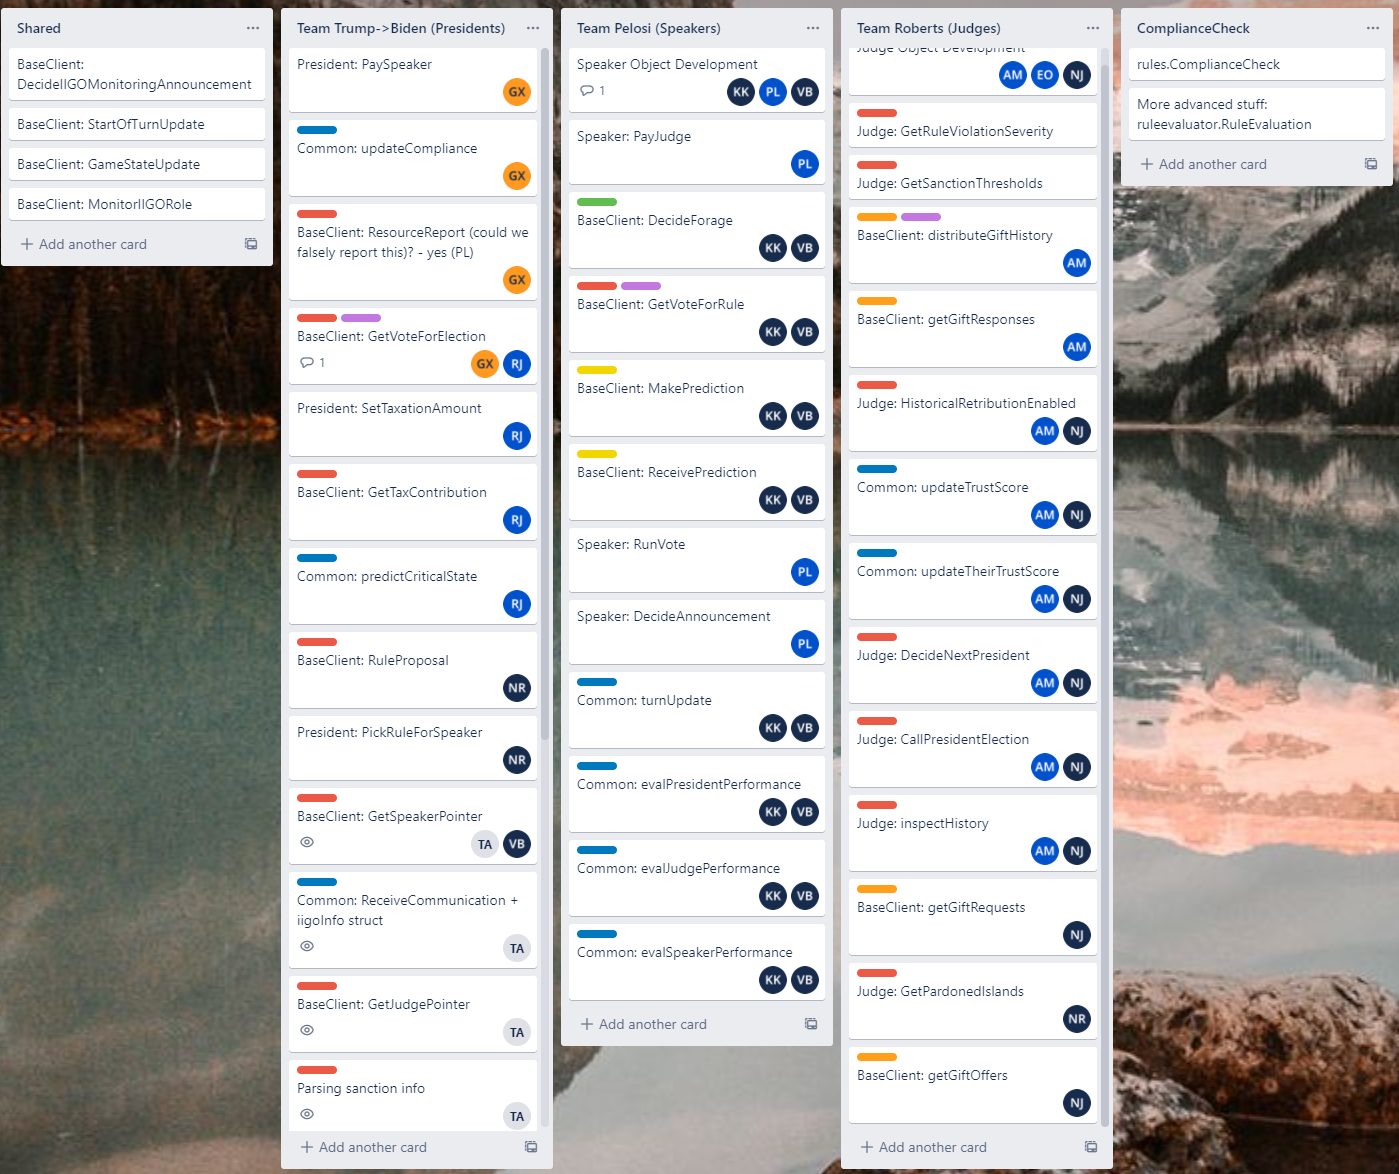
\includegraphics[width=\textwidth,height=\textheight,keepaspectratio]{11_team3_agentdesign/figures/post_mvp_trello.png}
    \caption{Screenshot of post-MVP agent strategy kanban Board.}
    \label{fig:post_mvp_trello}
\end{figure}